\graphicspath{{figures/chap01/}}

\chapter{引言}\label{chap:introduction}

\section{课题背景和意义}

%\subsection{非侵入式等离子体电子参数诊断}
\subsection{托卡马克等离子体的电子温度与密度诊断}

以未来大规模聚变能应用为目的,托卡马克高温聚变等离子体研究早已取得如等效 Q 值达 $1.25$\cite{JT60U:Q1.25} 以及 $16.1\,{\rm MW}$\cite{JET:NF:16MW:1,JET:NF:16MW:2} 的瞬时聚变功率输出等显著成果,国际热核聚变堆(ITER)的开工建设\cite{Holtkamp2007:ITER}成为托卡马克聚变研究一个新的里程碑。可控聚变研究的进步离不开等离子体诊断技术和工具的应用,可以说一个托卡马克装置的诊断能力直接决定了该装置物理研究的深度和运行表现。为了在托卡马克运行中实现等离子体的控制和研究,需要对数目众多的等离子体参数进行诊断测量,其中电子温度 $T_{\rm e}$ 与密度 $N_{\rm e}$ 是最基本也是最重要的物理量\cite{ITERPhysics:chap7}。

对于托卡马克边界温度较低的等离子体,静电探针(即朗谬尔 Langmuir 探针)\cite{LangmuirProbe}是广泛应用的一种诊断手段。静电探针利用等离子体的壳层理论,将一小段加入偏置电压的高熔点金属伸入等离子体,通过测量其伏安特性曲线即可得到等离子体的 $T_{\rm e}$ 和 $N_{\rm e}$ 参数,特别是静电三探针\cite{tripleprobe}的使用,将静电探针的应用范围进一步扩大。通过对静电探针的结构进行精心设计,还可以测量等离子体边界的很多其他物理信息\cite{LangmiurProbe-EdgeTurbulance,LangmiurProbe-ZonalFlow}。

对于托卡马克芯部的等离子体,其温度很高,
%托卡马克研究中等离子体的温度越来越高,
一些传统的,与等离子体有直接接触的诊断手段则显得不再适用,所以,
%在对
%托卡马克等离子体\pozhehao 特别是
%芯部等离子体
%\pozhehao
%的诊断中,
非侵入式(noninvasive)的诊断手段受到了重视。其中,一些方法主动地将“探针”粒子束或激光束从外部射入等离子体进行诊断,%为“主动”式的诊断手段,
而另一些方法%“被动”的诊断方法
则被动地接收测量从等离子体射出的粒子或辐射进行诊断。

对于“主动”式的诊断手段,主要通过
%将电磁波(或激光)探测束射入等离子体,通过
对探测束(粒子束、激光束或微波波束)与等离子体的相互作用进行等离子体参数的测量,主要包括但不限于以下几种诊断手段:
%诊断的方法主要有:

\hspace{0.25em}\textbullet\hspace{0.45em}可诊断 $T_{\rm e}$ 的激光汤姆逊散射(Thomson scattering)测量\cite{ThomsonScattering:1,ThomsonScattering:2,ThomsonScattering:3}

\hspace{0.25em}\textbullet\hspace{0.45em}可诊断 $N_{\rm e}$ 的微波折射(refractometry)测量\cite{refractometry}

\hspace{0.25em}\textbullet\hspace{0.45em}可诊断 $N_{\rm e}$ 的微波反射(reflectometry)测量\cite{MicrowaveReflectometry}

\hspace{0.25em}\textbullet\hspace{0.45em}可诊断 $N_{\rm e}$ 的微波\cite{MicrowaveInterferometry}(或激光\cite{LaserInterferometry})干涉(interferometry)测量

\hspace{0.25em}\textbullet\hspace{0.45em}可同时诊断 $T_{\rm e}$ 和 $N_{\rm e}$ 的束发射光谱(beam emission spectroscopy)\cite{Li-beam,Schmitz2008}测量

%而将探测粒子束从边界打入等离子体,探测该粒子束的谱线辐射可以同时确定等离子体的 。

%这些“主动”式的诊断手段,首先需要针对实验装置一套特定的探测束发生设备,然后对探测束的入射路径以及信号接收测量设备进行设计和安装调试,其诊断系统比较复杂,且诊断系统一般都需要进行特殊的设计和考虑。

%同时,
托卡马克等离子体具有自微波波段至 X 射线波段丰富的辐射,只需“被动”地接收测量这些辐射即可获得大量的等离子体信息,例如:辐射\cite{Bolometer:DIIID:radiatedPower,Bolometer:JET:radiatedPower}在 等离子体的能量平衡中起着重要作用;具有等离子体参数空间分辨诊断能力的束发射光谱法被广泛用来进行托卡马克边界物理研究\cite{BES:PPCF:1993};而对杂质或工质气体粒子的光谱测量可以用来研究杂质的输运行为\cite{HT7:CarbonTransport}、 粒子循环与输运物理\cite{ParticleTransport:PPCF:2009}等。其中,可以用于等离子体 $T_{\rm e}$ 和 $N_{\rm e}$ 诊断的方法主要有:

\hspace{0.25em}\textbullet\hspace{0.45em}可诊断 $T_{\rm e}$ 的 X 射线能谱测量\cite{Xray-spectrum-Te-Ti}

%\hspace{0.25em}\textbullet\hspace{0.45em}可诊断 $T_{\rm e}$ 的韧致辐射测量

\hspace{0.25em}\textbullet\hspace{0.45em}可诊断 $T_{\rm e}$ 的电子回旋辐射(electron cyclotron emission, ECE)测量\cite{ECE:physics}

\hspace{0.25em}\textbullet\hspace{0.45em}可诊断 $N_{\rm e}$ 的谱线斯塔克展宽(Stark broadening)测量\cite{Stark-broadening}

%ECE 等被动地测量等离子体的电子回旋辐射(Electron cyclotron emission, ECE)可以提供 $T_{\rm e}$ 参数的空间分布信息\cite{ECE:physics},然而 ECE 诊断的空间分辨能力随着等离子体温度的上升而下降\cite{ECE:high-temprature},且电子回旋辐射在等离子体内存在截止的问题,限制了对等离子体空间的诊断能力\cite{ECE:access-limit}。

在被动地接收等离子体辐射的诊断手段中,利用等离子体内原子特征谱线辐射强度比进行 $T_{\rm e}$ 和 $N_{\rm e}$ 同时测量的光谱诊断方法,是托卡马克等离子体研究中一种重要的诊断手段。该方法具有不干扰等离子体,光谱测量设备简单且不受复杂电磁环境的影响以及仅需进行相对标定的优点\cite{boivin2001,xie:wlxb},在大型托卡马克如 JET\cite{Davies1997-HeBES-JET} 和 JT-60U\cite{Hirotaka1999-HeCRM-JT60U} 等装置上取得了初步成果,在未来聚变等离子体研究中有着广阔的应用前景。

%\subsection{托卡马克等离子体电子温度 $T_{\rm e}$ 和电子密度 $n_{\rm e}$ 诊断}

%\subsection{原子发射光谱诊断}

\subsection{氦原子的能级特点与利用其发射光谱进行诊断的优势}

\begin{figure}
  \centering
  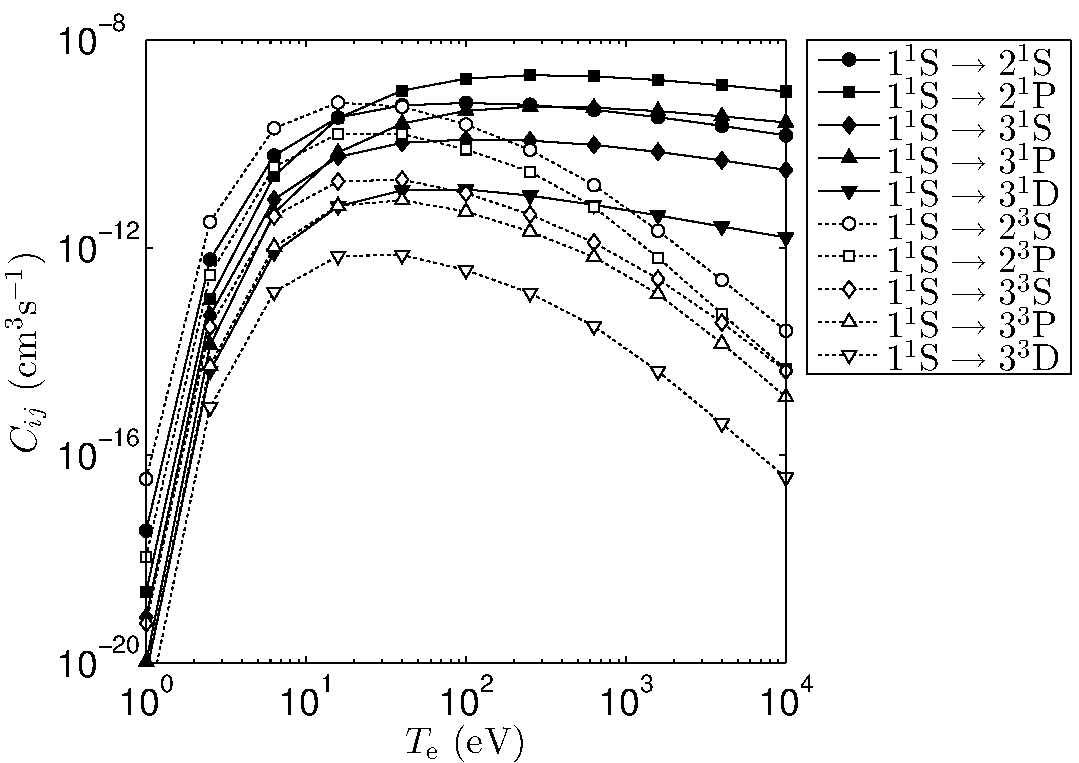
\includegraphics[height=0.35\textheight]{excRate-from-1.pdf}
  \caption{氦原子基态的电子碰撞激发速率系数,计算自 \onlinecite{Ralchenko2008603,NIFS:DATA:059} 的电子碰撞截面数据。}
  \label{fig:chap01:excRate:gs}
\end{figure}

氦原子的能级结构特点决定了其发射光谱适合用来进行托卡马克等离子体的诊断。

首先,氦原子能级结构拥有自旋单重态(singlet)和三重态(triplet)两套电子自旋系统。自旋三重态能级只能通过自旋变化过程激发产生,而自旋单重态能级主要通过自旋守恒过程从基态激发产生,不同自旋系统能级间的电子碰撞跃迁反应截面与相同自旋系统能级间电子碰撞跃迁的反应截面具有不同的随 $T_{\rm e}$ 的变化行为(图 \ref{fig:chap01:excRate:gs}--\ref{fig:chap01:excRate:metasinglet})。对于基态原子,当电子温度高于 $20\,{\rm eV}$ 时,自旋变化和自旋守恒过程的电子碰撞速率系数变化趋势开始有明显的差别(图 \ref{fig:chap01:excRate:gs}),自旋守恒激发过程的速率系数在 $T_{\rm e}$ 为几百电子伏时具有最高值,并且当 $T_{\rm e}$ 在 $50\,{\rm eV}$ 至 $1\,{\rm keV}$ 范围可以视为常数,而自旋变化过程的电子碰撞激发速率系数在 $T_{\rm e}\sim 20\,{\rm eV}$ 时达到最高值,随着 $T_{\rm e}$ 的升高大致按照 $T_{\rm e}^{-2}$ 的速率下降。氦原子亚稳态原子 $2^3{\rm S}$ 和 $2^1{\rm S}$ 的碰撞激发速率系数在图 \ref{fig:chap01:excRate:metatriplet} 和图 \ref{fig:chap01:excRate:metasinglet} 中画出。可见,亚稳态电子碰撞激发速率系数的最高值出现在比基态更低的 $T_{\rm e}$ 处。两亚稳态的自旋守恒激发速率系数分布更为平坦,而自旋变化过程的速率系数在 $T_{\rm e}<10\,{\rm eV}$ 时就开始下降。同时,图 \ref{fig:chap01:excRate:metatriplet} 中画出了 $2^3{\rm S}$ 至 $2^1{\rm S}$ 的电子碰撞跃迁速率系数,它大概是激发至主量子数 $n=3$ 自旋单重态能级速率系数的 $10$ 倍。所以,来自从不同自旋系统能级的谱线强度之比与 $T_{\rm e}$ 有较强的函数关系,而来自相同自旋系统能级的谱线强度比与 $N_{\rm e}$ 具有较强的函数关系,通过测量氦原子谱线辐射可以同时确定等离子体的 $T_{\rm e}$ 和 $N_{\rm e}$ 。

\begin{figure}
  \centering
  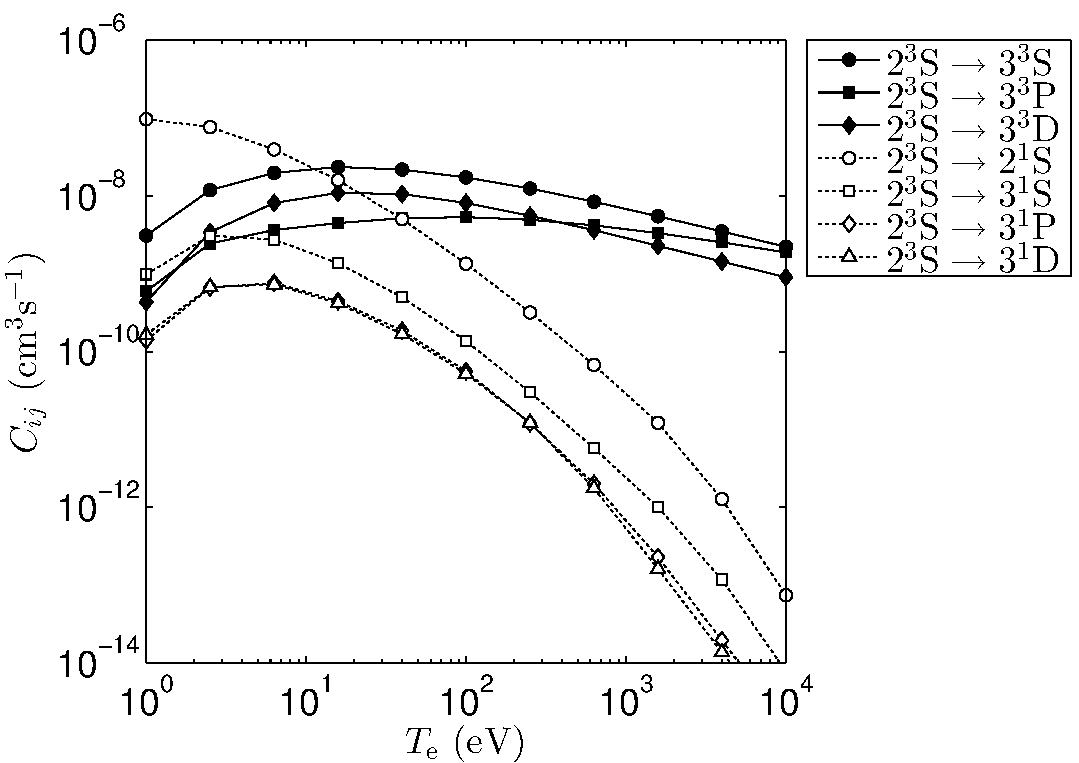
\includegraphics[height=0.35\textheight]{excRate-from-2.pdf}
  \caption{氦原子三重态亚稳态 $2^3{\rm S}$ 的电子碰撞激发速率系数,计算自 \onlinecite{Ralchenko2008603,NIFS:DATA:059} 的电子碰撞截面数据。}
  \label{fig:chap01:excRate:metatriplet}
\end{figure}

其次,在所有原子中,氦原子具有最高的基态电离能 $24.6\,{\rm eV}$。在氦原子束诊断托卡马克等离子体时,诊断束可以达到更深的位置,从而拓宽了诊断范围。

最后,氦为未来聚变等离子体中的固有元素,只需被动地测量氦原子的谱线辐射即可获得等离子体参数信息,不会给等离子体带来新的杂质粒子,即使现阶段大型托卡马克装置中利用氦束进行主动诊断,打入真空室的氦也不会对等离子体本身产生明显的影响\cite{Schmitz2008}。

因此,氦原子的发射光谱诊断(atomic emission spectroscopy)在高温聚变等离子体研究中得到了充分的重视,ITER 装置也已经考虑将氦原子的谱线诊断作为一种重要的诊断手段\cite{Mullane2002}。

\begin{figure}
  \centering
  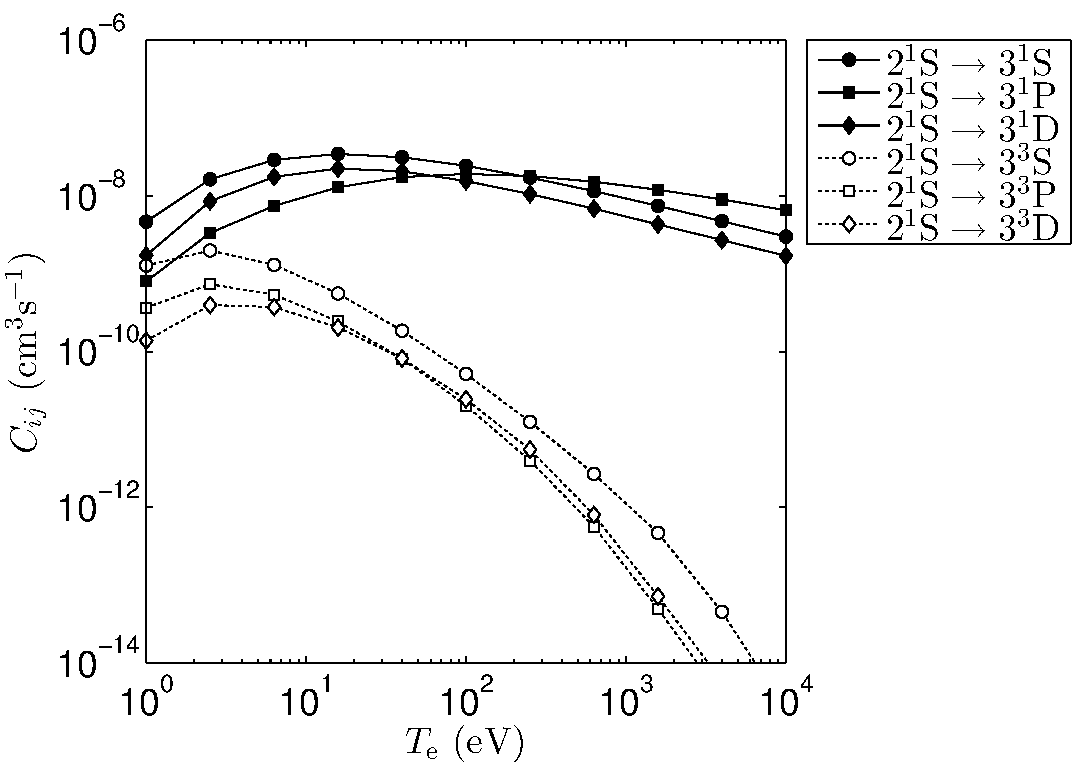
\includegraphics[height=0.35\textheight]{excRate-from-3.pdf}
  \caption{氦原子单重态亚稳态 $2^1{\rm S}$ 的电子碰撞激发速率系数,计算自 \onlinecite{Ralchenko2008603,NIFS:DATA:059} 的电子碰撞截面数据。}
  \label{fig:chap01:excRate:metasinglet}
\end{figure}


\subsection{氦原子发射光谱诊断的研究进展}
\label{sec:chap01:research-history}

最早提出使用自旋单重态和自旋三重态能级谱线辐射强度比方法测量等离子体电子温度的方法时
\cite{Sovie1964-He-coronal,Vries1966-He-coronal},是基于日冕模型(coronal model)的,后来研究中发现此方法只适用于电子密度很低的等离子体, 当 $N_{\rm e}$ 达到 $10^{11}\,{\rm cm}^{-3}$ 以上时,激发态的电子碰撞退激发过程对激发态数密度的影响加剧,此时应该使用碰撞辐射模型(collisional-radiative model)来计算激发态数密度分布\cite{Newe1966-He-CRRecommend}。

人们使用氦束发射光谱(beam emission spectroscopy)诊断等离子体参数是在 TEXTOR\cite{Schweer1992174} 上开始的。后来的类似诊断\cite{Davies1997-HeBES-JET,Field-HeBES-COMPASSD,Hidalgo-HeBES-TJII}
都使用了 TEXTOR 的碰撞辐射模型,该模型中考虑了包括基态在内的主量子数 $n\le 4$ 的共 19 个能级。当氦束为稳态束流时,本地局域的氦原子激发态数密度保持稳定,只与本地的 $T_{\rm e}$ 和 $N_{\rm e}$ 相关,氦束在等离子体中直线传播,当氦原子被碰撞电离后,即沿磁力线运动而离开束流区域,所以氦离子的复合过程可以忽略,这样用于氦束发射光谱诊断的碰撞辐射模型被大大简化。

后来在 MST 上进行了高速氦束(fast helium beam)发射谱线的诊断研究\cite{Ahn2007-He-BES},并对例如杂质、磁场和离子碰撞等因素对谱线的影响进行了讨论,模型采用了 ADAS\cite{ADAS} 的代码和截面数据,包含了众多能级($n\le 110$),对主量子数能级 $n\le5$ 的能级根据 $nlSL$ 分别处理,将更高能级自旋相同的能级简并。最近 TEXTOR 对模型进行了进一步发展\cite{Schmitz2008},包括了较高的能级粒子,并对重粒子碰撞跃迁和电荷交换过程进行了考虑。而 MAP-II 偏滤器模拟装置\cite{Iida2010-HeBES-MAPII}的束发射光谱诊断工作中使用了 M. Goto 的模型\cite{Goto2003-HeCRM},并对辐射在等离子体中的捕获效应进行了讨论。

\begin{table}
\caption{氦束发射光谱诊断等离子体参数实验及使用的碰撞辐射模型}
{\small nlSL:能级以 nlSL 区分;nS:能级以自旋角动量区分;n:能级仅以主量子数区分;e-He:电子碰撞过程;rad:辐射过程;CX:电荷交换过程;ion-ion/dblion:离子碰撞电离与双电子电离;ion-exc/deexc:离子碰撞激发与退激发;D-tran:氘输运过程;rad-trap:辐射俘获效应;Goto:与文献 \onlinecite{Goto2003-HeCRM} 相同。}
\label{tab:chap01:HeBES:CRM}
\begin{center}
\begin{tabular}{llllll}
\toprule[1.5pt]
       装置 & 区域 & 谱线能级 & 包含能级 & 包含过程 & 来源\\
\midrule[1pt]
    TEXTOR & 边界
            & $3^1{\rm D}$, $3^1{\rm S}$, $3^3{\rm S}$
            & $n\le4$
            & e-He, rad
            & \onlinecite{Schweer1992174} \\ \addlinespace[.5em]
    JET & 偏滤器
            & $3^1{\rm D}$, $3^1{\rm S}$, $3^3{\rm S}$
            & $n\le4$
            & e-He, rad
            & \onlinecite{Davies1997-HeBES-JET} \\ \addlinespace[.5em]
  COMPASS-D & 边界
            & $3^1{\rm D}$, $3^1{\rm S}$, $3^3{\rm S}$
            & $n\le4$
            & e-He, rad
            & \onlinecite{Field-HeBES-COMPASSD} \\ \addlinespace[.5em]
      TJ-II & 边界
            & $3^1{\rm D}$, $3^1{\rm S}$, $3^3{\rm S}$
            & $n\le4$
            & e-He, rad
            & \onlinecite{Hidalgo-HeBES-TJII} \\ \addlinespace[.5em]
    MST & 边界
            & $3^1{\rm D}$, $4^1{\rm D}$, $3^1{\rm P}$
            & \makecell[l]{nlSL: $n\le5$,\\
                nS: $6\le n\le 110$}
            & \makecell[l]{e-He, rad, CX\\
                ion-ion/dblion,\\ ion-exc/deexc}
            & \onlinecite{Ahn2007-He-BES} \\ \addlinespace[.5em]
    TEXTOR & 边界
            & $3^1{\rm D}$, $3^1{\rm S}$, $3^3{\rm S}$
            & \makecell[l]{nlSL: $n\le4$,\\
                nS: $5\le n\le 7$,\\
                n: $n=8, 9$, He$^+$}
            & \makecell[l]{e-He, rad, D-CX\\
                D-tran($\Delta n=0$)}
            & \onlinecite{Schmitz2008} \\ \addlinespace[.5em]
    MAP-II & \makecell[l]{偏滤器\\ 模拟装置}
            & \makecell[l]{$3^1{\rm D}$, $3^1{\rm P}$\\
                $4^3{\rm S}$, $3^3{\rm D}$, $3^3{\rm S}$}
            & Goto
            & Goto, rad-trap
            & \onlinecite{Iida2010-HeBES-MAPII} \\
\bottomrule[1.5pt]
\end{tabular}
\end{center}
\end{table}

表 \ref{tab:chap01:HeBES:CRM} 列出了用氦束发射光谱作为等离子体诊断手段的一些实验,这些实验主要集中在对边界和偏滤器等离子体的诊断,氦束发射光谱诊断法可以获得很高空间分辨率的 $T_{\rm e}$ 和 $N_{\rm e}$ 参数,对托卡马克等离子体的粒子输运、L--H 转换,MHD 约束行为的研究有很重要的作用。

在氦束发射光谱诊断的碰撞辐射模型处理上,一般忽略了离子对能级数密度的贡献。在氦(或混入氦气)等离子体中,氦离子的影响则不再可以忽略,T. Fujimoto\cite{Fujimoto1979-HeCR} 建立了适用于低温氦气放电等离子体($N_{\rm e}=6.3\times10^{10}\,{\rm cm}^{-3}$, $T_{\rm e}=6\,{\rm eV}$)的碰撞辐射模型。在每种不同的等离子体条件下,添加不同的过程或外界条件的影响,T. Fujimoto 的模型在实验中得到了充分的应用和验证。同时,M. Goto 分别在 1997\cite{Goto1997-HeCRM-WT3} 和2003\cite{Goto2003-HeCRM} 年根据最新的碰撞截面数据对此模型进行了修订和更新。基于此模型在一些等离子体中的诊断应用总结于表 \ref{tab:chap01:FujimotoHeCRM:applications} 中。

\begin{table}
\caption{T. Fujimoto 的碰撞辐射模型在不同等离子体条件下的应用}
{\small wall: 器壁猝熄过程(quenching at wall);meta-meta:亚稳态原子非线性碰撞过程;$\nu$-abs/exc/ion:辐射吸收、激发与电离过程;hot-e:射频加热产生的热电子效应;res-scat:辐射的共振散射效应(resonance scattering of radiation);ionizing condition: 激发态粒子数密度独立于 ${\rm He}^+$ 密度。}
%\vspace{-1.5em}
\label{tab:chap01:FujimotoHeCRM:applications}
\begin{center}
\begin{tabular}{llll}
\toprule[1.5pt]
       装置 & 等离子体条件 & 添加过程或实验技术 & 来源\\
\midrule[1pt]
     - & 辉光放电
            & \makecell[l]{wall, meta-meta,\\ $\nu$-abs/exc/ion}
            & \onlinecite{Fujimoto1979-HeCR} \\ \addlinespace[.5em]
   NAGDIS-I & 氦等离子体
            & \makecell[l]{hot-e, res-scat}
            & \onlinecite{Sasaki1996-HeCRM-NAGDIS} \\ \addlinespace[.5em]
   JT-60U & \makecell[l]{偏滤器再循环氦}
            & \makecell[l]{ionizing condition}
            & \onlinecite{Hirotaka1999-HeCRM-JT60U} \\ \addlinespace[.5em]
   WT-3 & \makecell[l]{10\% 混氦}
            & \makecell[l]{$L-S$ 耦合}
            & \onlinecite{Goto1997-HeCRM-WT3} \\ \addlinespace[.5em]
   LHD & \makecell[l]{混氦}
            & \makecell[l]{$L-S$ 耦合}
            & \onlinecite{Goto2003-HeCRM} \\ \addlinespace[.5em]
  HYBTOK-II & \makecell[l]{氦等离子体}
            & \makecell[l]{CCD 相机 2 维测量}
            & \onlinecite{Ohno2010-HeCRM-2D-measure} \\
  H-1 & \makecell[l]{混氦}
            & \makecell[l]{计算机断层重建}
            & \onlinecite{MaShuiliang2012:Tomography} \\
\bottomrule[1.5pt]
\end{tabular}
\end{center}
\end{table}

从谱线强度比数据中分析出等离子体 $T_{\rm e}$ 和 $N_{\rm e}$ 的过程以碰撞辐射模型对等离子体谱线强度比与$T_{\rm e}$ 和 $N_{\rm e}$ 之间关系的计算为基础
\cite{Fujimoto1979-HeCR,Goto2003-HeCRM,boivin2001},碰撞辐射模型的建立包括选取模型包含的激发态能级,对能级之间电子碰撞反应过程的处理以及这些反应过程的速率系数(反应截面)的计算,在实际工作中,这些因素都会对模型的计算结果产生影响。早期的工作中\cite{Fujimoto1979-HeCR},人们期待在碰撞辐射模型中加入足够多的反应能级和碰撞辐射过程来满足计算结果的有效性,但由于包含的激发态能级不同,以及使用的速率系数精度较低\cite{Summers:IAEAdatarequirement},不同模型的计算结果差别较大
\cite{Boivin2007}。后来,M. Goto\cite{Goto2003-HeCRM}尝试更新模型的反应速率系数以获得精度更高的计算结果,同时 Y. Andrew 等人\cite{Andrew2000PPCFSensitivity}计算了模型中反应速率系数的不确定度对计算结果的影响,在 O. Schmitz 等人\cite{Schmitz2008}的工作中,将氦谱线比的诊断结果与其他诊断手段的结果进行对比来验证谱线比法诊断结果的有效性。

\begin{figure}%[H]
  \centering
  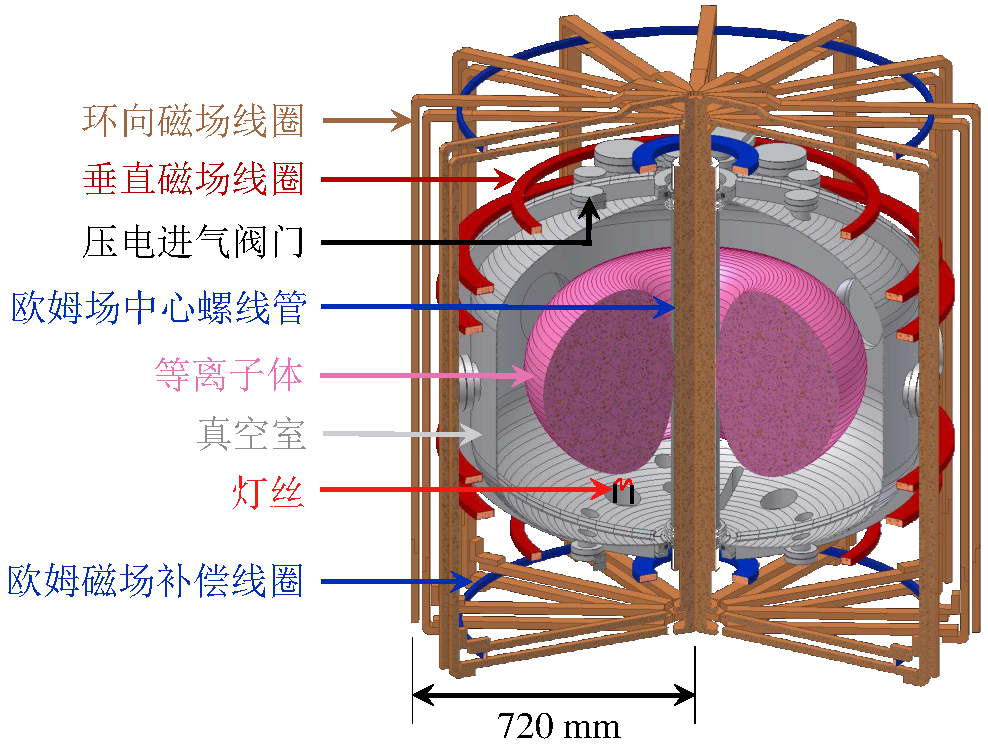
\includegraphics[width=0.8\textwidth]{SUNIST-Sketch-14_cropped.pdf}
  \caption{SUNIST 装置示意图,修改自\onlinecite{sunist:sketch:wiki}}
  \label{fig:chap01:sunist-sketch}
\end{figure}

%\subsection{国内研究现状}
\subsection{国内托卡马克等离子体的光谱诊断研究}

国内的托卡马克研究者也进行了大量的光谱诊断工作。在 CT-6B 装置中,李赞良等人\cite{LiZanliang:CT-6B:Te} 在 1989 年通过氧离子的真空紫外光谱测量了电流上升阶段的电子温度;后来赵庆勋等人\cite{ZhaoQingxun:CT-6B:Rotate}在 1997 年根据 OII $464.2\,{\rm nm}$、CIII $464.7\,{\rm nm}$ 和 ${\rm H}_\alpha$ 谱线的多普勒位移,测量了等离子体极向转动速度的径向分布。在 HT-7 装置上,刘建坤\cite{LiuJiankun2001:HT-7:PDA}等人使用光电二极管阵列,测量了 ${\rm H}_\alpha/{\rm D}_\alpha$ 的光谱,对粒子约束时间进行了系统研究;周倩等人\cite{ZhouQian2005:HT-7:carbon}在 2005 年通过对碳杂质的谱线辐射进行空间分辨测量,研究了碳杂质在径向的输运行为并在 2007 年完善了用于轻杂质粒子输运研究的光谱诊断系统;2010 年 HT-7 上用于电荷交换复合光谱诊断的诊断中心束束系统建成,实现了离子温度剖面分布测量\cite{ShiYuejiang2010:HT-7:CXRS};同时,陈开云等人\cite{ChenKaiyun2009:HT-7:SXTomography} 在 HT-7 上开展了基于断层扫描技术的软 X 射线诊断工作。在 J-TEXT 装置上通过测量软 X 射线辐射进行了反锯齿行为(inverse sawtooth activity)的研究\cite{FengXD2013:J-TEXT:softxray}。 崔正英等人\cite{CuiZhengying:2010:VUV}在 HL-2A 装置上建立了具有空间分辨诊断能力的真空紫外光谱测量系统,可以用于边界杂质和温度分布的测量。在 EAST 装置上,新建立了充气成像系统(gas puffing imaging),此系统可以有效的测量等离子体边界的湍流结构\cite{LiuSC:2012:EASTGPI},利用此系统成功研究了 L--H 转换的中间振荡过程(intermediate oscillatory phase)\cite{XuGS2014:EASTGPI:L-I-H}。

由此可见,虽然国内托卡马克光谱诊断研究众多,但基于碰撞辐射模型,通过测量原子谱线辐射强度比的方法诊断 $T_{\rm e}$ 和 $N_{\rm e}$ 参数的研究在国内尚未见报道。而低温等离子体研究领域,国内的研究者处于领先水平\cite{ZhuXM2010:Review}。通过低温等离子体可见光谱辐射诊断的研究\cite{ZhuXM2009:Thesis}发现,根据等离子体条件做必要的假设,通过在碰撞辐射模型中包含最主要的粒子和过程,可以对谱线比法诊断等离子体进行有效的指导。

\subsection{SUNIST 装置、等离子体参数范围与诊断需求}

\begin{figure}%[H]
  \centering
  \begin{overpic}[width=0.6\textwidth]{sunist_parram_vs_lineratio_range_2.pdf}
    \put(45,34){氦谱线比法}
	\put(51,45){SUNIST}
  \end{overpic}
  %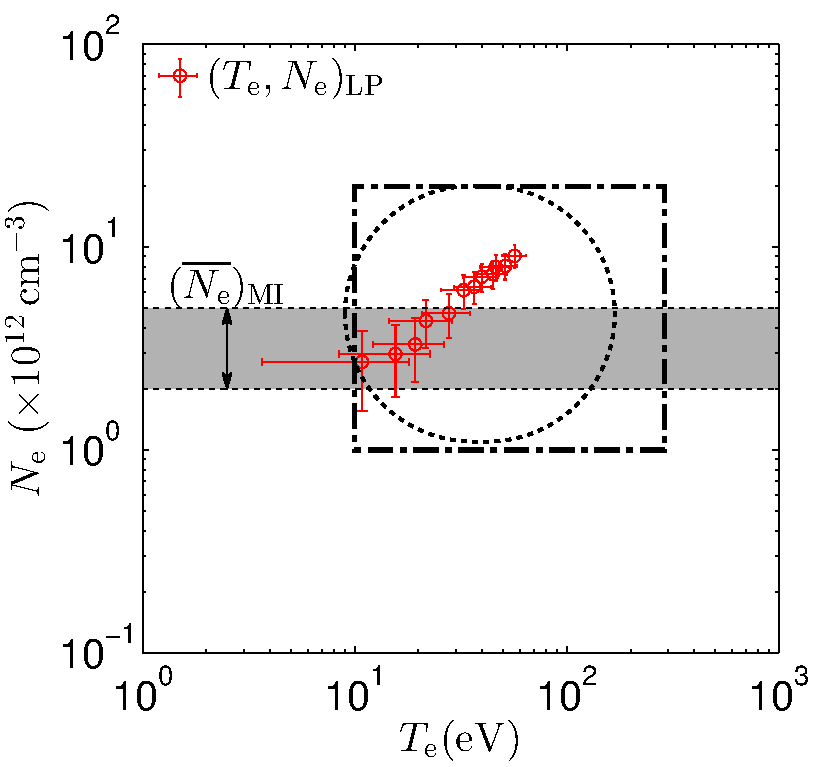
\includegraphics[width=0.6\textwidth]{sunist_parram_vs_lineratio_range_2.pdf}
  \caption{氦谱线比法诊断适用的电子参数范围与 SUNIST 等离子体参数范围估计。$(T_{\rm e},N_{\rm e})_{\rm LP}$ 表示静电探针测量的边界等离子体参数\cite{WangWH2005:PPCF:Edge};$(\overline{N_{\rm e}})_{\rm MI}$ 表示微波干涉仪测量的电子密度范围值(第 \ref{sec:chap04:lineratio-ne-te} 节)。点划线表示氦原子谱线比法的适用范围;点线表示 SUNIST 等离子体电子参数估计范围。}
  \label{fig:chap01:te-ne-range}
\end{figure}

中国联合球形托卡马克(Sino-UNIted Spherical Tokamak,SUNIST)是我国第一台,也是唯一一台球形托卡马克装置\cite{Heyexi2002:SUNIST},图 \ref{fig:chap01:sunist-sketch} 所示为 SUNIST 装置示意图。

SUNIST 装置的主要参数为:大半径 $R_0=0.3\,{\rm m}$,小半径 $a=0.23\,{\rm m}$,欧姆放电时的等离子体电流 $I_{\rm p}\sim50\,{\rm kA}$,边界电子温度 $T_{\rm e}=20\sim100\,{\rm eV}$ 和电子密度 $N_{\rm e}=1\sim10\times10^{12}\,{\rm cm}^{-3}$\cite{WangWH2005:PPCF:Edge}(SUNIST 放电时的电子参数范围估计如图 \ref{fig:chap01:te-ne-range} 所示),真空室本底气压$p_{\rm gas,b}\sim5\times10^{-5}\,{\rm Pa}$,氦气放电充气气压范围 $p_{\rm gas}=2\sim5\times10^{-3}\,{\rm Pa}$。

%SUNIST 实验中,传统的等离子体电子参数诊断手段也面临着挑战,如静电探针会被高温等离子体烧蚀(图 \ref{fig:chap01:ProbeVapor}),这不但会缩短静电探针的使用寿命,而且会为诊断数据解析带来困难,烧蚀释放的重元素杂质粒子也会污染等离子体;同时,
SUNIST 做为小型球形托卡马克实验装置,研究人员匮乏,所以 SUNIST 装置亟需部署低成本、不干扰等离子体、少维护或免维护的可靠诊断手段。

%\begin{figure}%[H]
%  \centering
%  %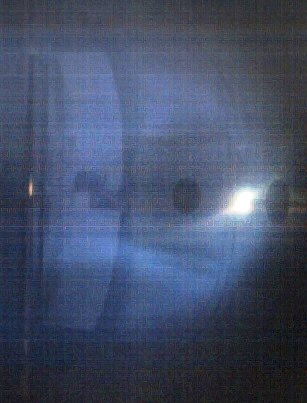
\includegraphics[height=0.3\textheight]{ProbeVapor121123020.jpg}
%  \begin{overpic}[scale=0.7]{ProbeVapor121123020-bw.jpg}
%    \put(1,22){\color{white}{\bf 中心柱}}
%    \put(2,29){\color{white}{$\uparrow$}}
%
%    \put(25,87){\color{white}{\bf 等离子体}}
%    \put(35,80){\color{white}{$\downarrow$}}
%
%    \put(50,59){\color{white}{\bf 静电探针}}
%    \put(67,53){\color{white}{$\downarrow$}}
%
%    \put(50,33){\color{white}{\bf 烧蚀亮点}}
%    \put(58,40){\color{white}{$\uparrow$}}
%  \end{overpic}
%  \caption{SUNIST放电时静电探针烧蚀情况(炮号:121123020)}
%  \label{fig:chap01:ProbeVapor}
%\end{figure}

\subsection{课题意义}
\label{sec:ketiyiyi}

利用等离子体的谱线辐射强度比进行诊断的方法具有不干扰等离子体,光谱测量设备简单且不受复杂电磁环境的影响以及仅需进行相对标定的优点。作为聚变产物,氦在聚变等离子体实验装置中是一种固有元素。所以利用氦原子谱线辐射强度比进行电子参数诊断不会为等离子体带入新的杂质,在高温聚变等离子体研究中得到了充分的重视。

然而,根据氦原子的谱线强度分析出 $T_{\rm e}$ 和 $N_{\rm e}$ 是以碰撞辐射模型对氦原子激发态数密度的计算为基础的。原子反应速率系数和碰撞辐射模型中包含的能级以及反应过程是影响碰撞辐射模型计算精度的主要因素。
%现阶段原子反应速率系数(或截面)数据主要有以下三种来源:实验测量
%\cite{Shah1988:ionizaiton-data-measure,Long1970:PhysRevA.1.260,Dixon1976}、
%理论计算\cite{CCCmethod,Sawey199381}与半经验公式拟合\cite{Fujimoto:IPPJ-AM-8},并且有人对此专门做过总结
%\cite{IAEA:Data:vol3,deHeer:INDC,Kato:NIFS:DATA:346}。然而这些数据来源的精度难以保证\cite{Ralchenko2008603},导致不同来源原子反应数据的碰撞辐射其计算结果也不尽相同\cite{Delabie2010:consistency}。%如第 \ref{sec:chap01:research-history} 节所述,
%为了得到更高精度的计算结果,人们往往在碰撞辐射模型中加入更多的能级粒子、反应过程以及可以对原子能级产生影响的因素。但因为使用的截面数据精度不一,导致碰撞辐射模型中包含更多的能级和反应过程时,并不能如预期那样获得更高精度的计算结果(第 \ref{sec:chap02:crm-problem} 节)。
%而且,
碰撞辐射模型中包含着众多的能级粒子和复杂的反应过程,且相互耦合,现并无有效的手段对碰撞截面数据不确定性到粒子数计算误差的传递进行有效计算的手段,也就无法对不同原子反应过程的数据提出具体的精度要求。
随着原子能级的升高,其原子数密度快速下降,在碰撞辐射模型中的重要性也随之下降。随之带来的问题是,在特定的等离子体参数条件下,碰撞辐射模型中包含至多高能级的激发态能级才能满足光谱诊断研究对精度的要求。
%或者由碰撞辐射模型中包含粒子数精简带来的误差会小于由原子反应速率系数精度的限制所带来的误差。

以上问题在托卡马克等离子体氦原子谱线比诊断的文献中鲜有报道。在低温等离子体研究领域,人们意识到这个问题\cite{ZhuXM2009:Thesis},并尝试在碰撞辐射模型中只包含与感兴趣能级粒子相关的主要过程,通过与实验的对比,来验证碰撞辐射模型的有效性。

在高温等离子体氦发射光谱诊断等离子体参数的实验中,适用的等离子体参数范围\cite{Schmitz2008} 为:$20\,{\rm eV}<T_{\rm e}<300\,{\rm eV}$ 与 $10^{12}\,{\rm cm}^{-3}<N_{\rm e}<2\times10^{12}\,{\rm cm}^{-3}$,这与 SUNIST 整个等离子体区域的参数范围一致(如图 \ref{fig:chap01:te-ne-range} 所示)。做为一台小型托卡马克装置,SUNIST 具有实验安排灵活的优势,适合进行诊断原理的验证性研究。
因此,我们在 SUNIST 中开展了氦原子光谱诊断研究。本文将根据 SUNIST 氦放电等离子体的特点建立碰撞辐射模型,研究影响模型计算结果的因素,包括速率系数不确定性和碰撞辐射模型中包含的能级粒子的影响等;验证利用氦原子谱线辐射强度比诊断 SUNIST 等离子体参数物理和技术上的可行性;并且在研究工作中为 SUNIST 完善运行设施,建立起光谱诊断系统,积累光谱诊断经验;同时,也希望为其他托卡马克装置采用此诊断提供参考。%奠定基础。

\section{本文研究思路、内容和结构}

\begin{figure}%[H]
  \centering
  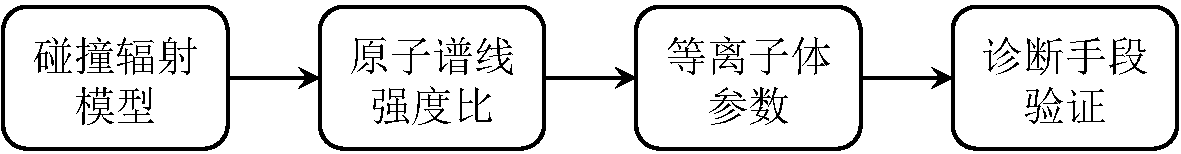
\includegraphics[width=0.8\textwidth]{research-progress.pdf}
  \caption{本论文研究过程图}
  \label{fig:chap01:research-progress}
\end{figure}

\begin{figure}%[H]
  \centering
  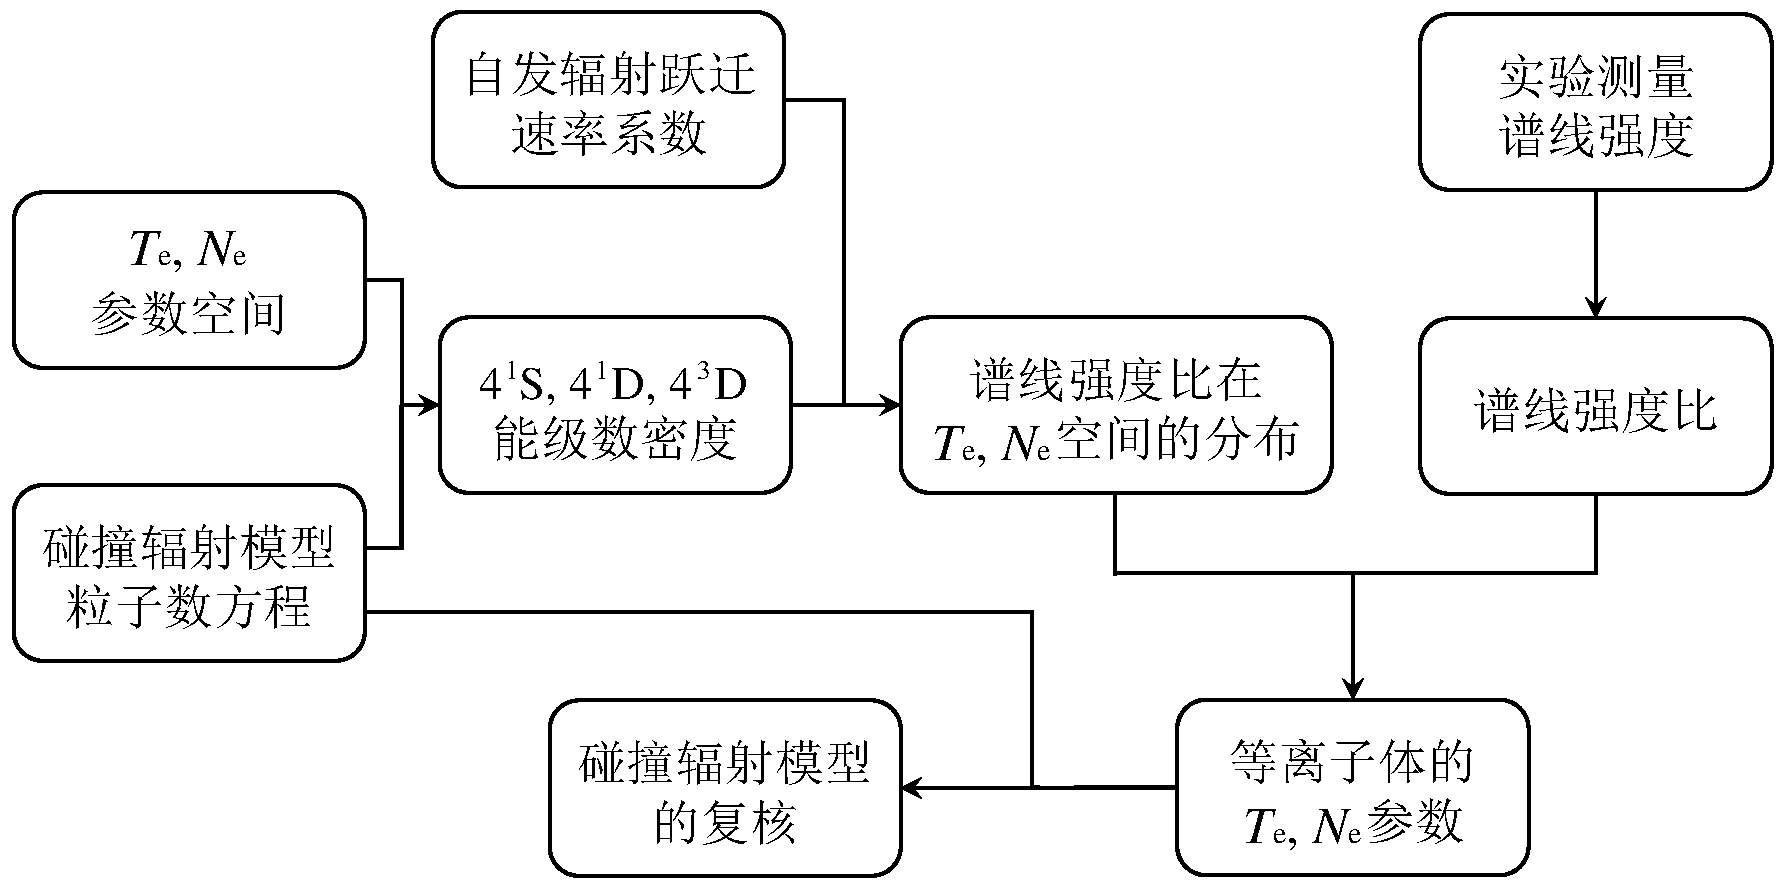
\includegraphics[width=\textwidth]{lineratio-method-rellevelabun.pdf}
  \caption{各部分研究内容的关系}
  \label{fig:chap01:research-relationship}
\end{figure}

本文以氦放电等离子体的原子发射光谱诊断 $T_{\rm e}$ 和 $N_{\rm e}$ 为对象,完成了碰撞辐射模型的建立、实验系统建设、诊断方法的建立和验证等研究内容。图 \ref{fig:chap01:research-progress} 和图 \ref{fig:chap01:research-relationship} 分别显示的是本论文研究过程图和各部分研究内容之间的关系。

论文首先建立适用于 SUNIST 氦放电等离子体的碰撞辐射模型,然后根据模型对谱线比的预测与实验测量进行对比得到等离子体的 $T_{\rm e}$ 和 $N_{\rm e}$ 参数,最后验证该方法的有效性,并针对影响诊断结果的因素进行讨论。

在碰撞辐射模型方面,首先分析了 SUNIST 等离子体参数下的氦原子激发态数密度分布特点,选定模型粒子数密度方程中包含的激发态能级和反应过程,并选择合适的反应截面数据进行计算。该部分是光谱诊断的基础,为从谱线强度测量数据获得相应等离子体参数提供谱线强度比预测结果。

碰撞辐射模型在特定的等离子体参数空间提供了原子谱线强度比的预测结果,而通过实验数据获得对应参数则是一个反过程。为了获得实验数据,课题工作中建立了相应的光谱诊断设备,对单色仪各项参数进行了标定,并尽最大限度对光电倍增管的信号信号和干扰做了消除减弱。%首先需要对 SUNIST 的放电控制进行优化。同时需要建立起相应的实验测量设备,包括实验数据采集以及光谱诊断设备等。

对发射光谱法诊断手段的验证内容手段有:在诊断得到的等离子体参数下,模型计算的激发态能级数密度和实验测量对比对碰撞辐射模型的复核;影响模型对谱线比预测结果的因素\pozhehao 包括能级的选取、速率系数的不确定性等\pozhehao 的分析;以及光谱测量的弦积分特性带来的误差的分析等。

%论文各部分内容的关系如下(图 \ref{fig:chap01:research-relationship}):1)在给定的等离子体参数空间内,利用碰撞辐射模型给出的粒子数方程计算出谱线比方法感兴趣能级的数密度;2)将有效自发辐射跃迁速率系数与能级数密度相乘,得到氦原子谱线强度,进而计算出谱线强度比在等离子体参数空间的分布;3)把实验测得的谱线数据与光谱仪响应的标定结果相结合,得到实验测量的谱线强度比;4)将碰撞辐射模型计算与实验测量的谱线强度比进行对比,得到等离子体的具体 $T_{\rm e}$ 与 $N_{\rm e}$ 参数;5)在获得的 $T_{\rm e}$ 与 $N_{\rm e}$ 参数下,可以用碰撞辐射模型计算出所有实验中测量的谱线激发态能级的数密度,将其与实验测量数据计算得到的激发态数密度进行对比,复核碰撞辐射模型对等离子体中的碰撞与辐射过程描述。

通过氦原子谱线辐射诊断 $T_{\rm e}$ 和 $N_{\rm e}$ 的工作,本文建立了从模型建立到实验测量,再到数据分析以及对诊断结果进行评估的整体框架。

本文结构如下:

第 \ref{chap:introduction} 章阐述了托卡马克高温聚变等离子体中光谱发射诊断研究的概况,介绍了本文研究的意义,给出了论文的主要研究内容和安排。

第 \ref{chap:crm-intro} 章从光子产生至被光谱系统检测测量所经历的物理过程出发,分析了影响谱线强度的因素:自发辐射跃迁几率、光子在等离子体内的传输以及自发辐射跃迁上能级激发态粒子数密度。给出了日冕、碰撞辐射模型和局域热平衡三种主要描述等离子体内粒子数密度分布的模型。介绍了高温聚变等离子体研究中使用的碰撞辐射模型的一般处理方法,并在最后指出现阶段氦原子谱线比诊断研究中使用的碰撞辐射模型所存在的一些问题,即反应速率系数不确定性至激发态数密度的传递估计手段不明确,以及模型中应包含的粒子和反应过程缺乏系统研究。

第 \ref{chap:crmodel} 章通过分析 SUNIST 氦放电等离子体内氦原子的特点(如原子能级数密度分布特点、等离子体的光学厚度、杂质影响和多种过程的时间常数等)建立了相应的碰撞辐射模型。通过选取使用前人整理的碰撞反应截面数据,求解了模型结果并与 FLYCHK 代码包的计算结果进行对比。最后,根据 SUNIST 氦放点等离子体的实验测量选取合适的谱线比,建立了氦原子谱线比诊断电子温度和密度的方法。

第 \ref{chap:measureing-system} 章介绍了 SUNIST 上的光谱诊断系统,包括光谱测量系统和测量路径安排,单色仪的谱线准确性、分辨率以及测量系统光谱响应的标定结果等。同时,介绍了降低信号噪声和消除基线干扰的手段,给出了 SUNIST 上基于重复放电的光谱测量手段以及氦原子谱线测量结果。相同的控制条件下 SUNIST 放电重复性的保证是测量的前提,本章也介绍了对提高放电重复性所做的研究,通过设计和安装 SUNIST 进气系统,改善了 SUNIST 放电的重复性。

第 \ref{chap:experiment} 章给出了 SUNIST 氦放电等离子体的光谱测量和等离子体电子温度与密度的诊断结果。通过其他未使用谱线对应激发态能级粒子数密度与碰撞辐射模型计算结果的对比,复核了本文建立的碰撞辐射模型。研究中还观察到弦积分光谱测量诊断的电子密度与微波干涉仪测量的弦平均电子密度的比值与电子参数剖面分布的峰化与否有直接关系、原子谱线强度与磁探针信号具有相同的涨落行为等结果,这为今后丰富和深入光谱诊断研究内容提供了参考和指引。

第 \ref{chap:summary} 章对本课题研究工作进行总结,指出工作的不足之处,并对未来的光谱诊断研究工作进行展望。

